\section{Decorating Sequences}
\label{sec:Decorating Sequences}
This chapter explores how to process Sequences by implementing the Decorator 
Pattern and effectively managing Sequence state. Discover powerful techniques 
to enhance Sequence functionality and manipulate data.

\subsection{Decorator Pattern}
\label{sub:Decorator Pattern}
% TODO Zitat von Gang of four
% TODO Quelle
Let us look at the Decorator Pattern~\cite{} to understand the content of the 
following sections. In object-oriented programming, the Decorator Pattern is a 
widely used concept. An object decorates another, as the name implies. As a 
result, an outer object refers to an inner object, and both implement the same 
interface. Therefore, the outer object forwards requests to the inner one. It 
modifies the calls on demand to manipulate or decorate the functionality of the 
inner one. Figure \ref{fig:seq_diagramm} shows how a decorator forwards the receiving calls and 
transfers the answer back to the client.

% TODO: replace
\begin{figure}[H]
    \centering
    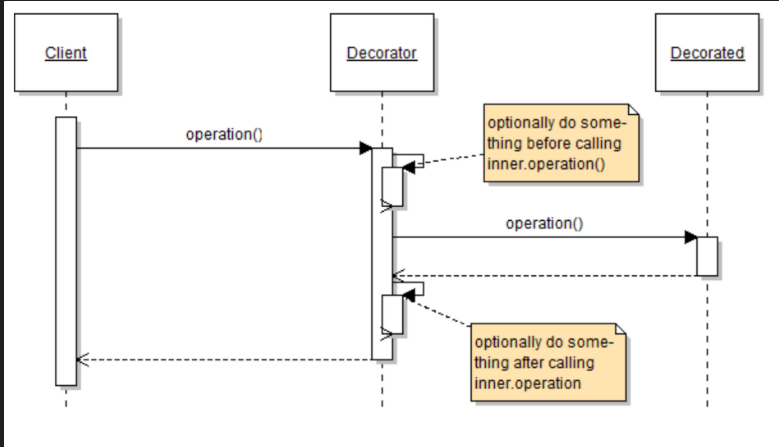
\includegraphics[width=0.8\textwidth]{./mainmatter/pictures/decorator_sequence_diagramm.png}
    \caption{Decorator Patter Sequence Diagram}
    \label{fig:seq_diagramm}
\end{figure}

The Decorator Pattern is often used in object-oriented programming languages 
because it adds additional functionality to an object at runtime. It is also 
possible to add extended functionality to a single class object. In the 
following, we will see how to exploit this to manipulate and change an Iterable.

\subsection{Processing Sequences}
\label{sec:Processing Sequences}
We use precisely that decorating approach to process Sequences further. 
The goal is to find a way to manipulate sequences so that they can solve 
complex problems. With many other programming languages, it is possible to write 
programs this way. Lists and operations on lists solve numerous problems in 
computer science. This way of programming has the advantage that the structure 
of the code is declarative. This code is more straightforward to understand 
and easier to extend.

\subsubsection{Manipulate Iteratbles with Functions}
\label{subsub:Manipulate Iteratbles with Functions}
In the following, |map| serves as a representative for any function of the
Sequence library. We call these functions in the following operators.
According to the package they are in.
Listing~\ref{lst:impl_map} shows how |map| processes a 
Sequence. For this, we use the Decorator approach just mentioned. To keep the 
example simple, on Line~\ref{line:seq_definition}, a client calls the map 
operator with a Sequence of numbers. However, it could process any iterable.
\newline
On line~\ref{line:args}, the function signature shows that a client can invoke 
|map| with two arguments: a mapper-function capable of processing an element of 
an iterable and an iterable. An iterable must adhere to the JS iterator protocol 
outlined in Section~\ref{subsub:The Iterable Protocol}. As a result, |map| can 
process Sequences, Arrays, or any other iterable. 

\begin{lstlisting}[
  style=ES6, 
  caption=Implementation of map,
  label={lst:impl_map}
  ]
const map = mapper => iterable => { *'\label{line:args}'*
*'\label{line:state_iterable}'*
const mapIterator = () => {
   const inner = iteratorOf(iterable);*'\label{line:state_iterator}'*
   let mappedValue;
 
   const next = () => {
     const { done, value } = inner.next();*'\label{line:inner_next}'*
     if (!done) mappedValue = mapper(value);
 
     return { /**@type boolean */ done, value: mappedValue }
   };
 
   return { next };
  };
 
  return createMonadicSequence(mapIterator);
};

const sequence = Sequence(0, x => x < 10, x => x++);*'\label{line:seq_definition}'*
const mapped   = map(x => x * 2)(sequence);*'\label{line:obj_mapped}'*
\end{lstlisting}

Because |map| decorates iterables, |map| also returns an object of type |Iterable<T>|. 
We define this object on line~\ref{line:obj_mapped} as |mapped|. 
Consequently, |map| also has a next function. Since the Iterable protocol 
specifies only this single function, it is the only one that must be externally 
callable. The object mapped now forwards function calls of the |next| function to 
the inner iterable, on line~\ref{line:inner_next}. The |mapper| function then 
processes the result and returns it.

\subsection{Benefits form the Decorater Approach}
\label{sub:Benefits form the Decorater Approach}
This section discusses the benefits and consequences of using the Decorator 
Pattern to implement the Sequence library.

\subsubsection{Standalone Functions}
\label{subsub:Standalone Functions}
In an object-oriented approach, the Sequence object defines the operators to 
process the elements. Therefore, such operators are available by using dot notation. 
Similar to Java implements the Stream API \cite{noauthor_stream_nodate}. 
However, with the approach of programming the operators independently, there 
are three significant advantages:

\begin{enumerate}
  \item {Strict adherence to the open-close principle. Changes to an operator do
      not affect the implementation of Sequence. Also, extensions to the 
      Sequence library do not affect existing code.
    }
  \item{Adherence to the single responsibility approach. The Sequence 
      constructor has only the task of creating a sequence. Mapping the
    elements of a sequence is not its responsibility.
  }
  \item{Easy scalability is guaranteed. It is very straightforward to add new 
    functionality from the outside.
  }
\end{enumerate}

Due to the independent implementation of the iterable operators, the last 
parameter can be the iterable object. The operator, therefore, defines the 
parameters in a curried style. So it is possible to benefit from eta-reduction 
in different situations.

\subsection{Stateful Decorating}
\label{sub:Stateful Decorating}
A state is present as soon as operators decorate iterables or implement 
additional functionalities. This chapter is about where the operators implement 
this state and which consequences this implies.

There are two possibilities for including the state.
Both variants are possible and are the content of the following two scenarios. 
The first scenario places the state into the closure scope to the surrounding 
operator of the iterator. The second scenario implements the state into the 
closure scope of the iterator. For both variants, it is of great relevance that 
the underlying object must not be changed.

\subsubsection{Scenario 1}
Listing~\ref{lst:scen_1} shows that the state is on line~\ref{line:scen_1_state}.
The state is created by calling SampleIterator and is valid for the entire 
object's lifetime. 

\begin{lstlisting}[
  style=ES6, 
  caption=Scenario 1 - State in closure scope of iterable,
  label={lst:scen_1}
  ]
const SampleIterable = () => {

  let i = 0; *'\label{line:scen_1_state}'*
  const next = () => {
    return { done: i > 5, value: i++ };
  };

  const copy = ...

  return {[Symbol.iterator]: () => ({ next })}
};
\end{lstlisting}

Listing~\ref{lst:scen_1_demo} shows a possible program flow. An object is 
created and then partially processed. On line~\ref{line:scen1_map} |map| also 
uses the same object. Line~\ref{line:scen1_output} shows an expected result. 
Nevertheless, copying the object before processing is necessary to achieve this 
result. That implies that each sequence must be copyable. Generating a new 
sequence with the same parameters allows for creating a copy of the sequence. 
The same is true for any function that decorates an iterable.

\begin{lstlisting}[
  style=ES6, 
  caption=Scenario 1 - Example usage,
  label={lst:scen_1_demo}
  ]
const seq = SampleIterable(0, x => x < 5, x => x++); // [0, 1, 2, 3, 4]
const mapped = map(id)(seq); *'\label{line:scen1_map}'*

for (const elem of mapped) {
  break; // Just consuming one element
}
for (const elem of seq) {
  console.log(elem);
}
// => Logs: '[0, 1, 2, 3, 4]' *'\label{line:scen1_output}'*
\end{lstlisting}

In many respects, copying is an elaborate thing. All operators and constructors 
dealing with sequences must implement it. Thus, implementation errors are 
possible. On the other hand, it is also an extra effort from a performance point 
of view. It means more function calls and also giant stack calls to manage.
The advantage of this implementation is that partially processed iterators could 
be further used with the current state because they do not reinitialize the 
state with a new iteration.
Because all objects must have copy implemented, operators can 
only process objects that implement copy. That means JavaScipt array or HTML 
Collection would not be processable.

\subsubsection{Scenario 2}
Listing~\ref{lst:scen_2} represents scenario 2. Here, the state is on 
line~\ref{line:scen_2_state}. Running the code from the previously
Listing~\ref{lst:scen_1_demo} produces the same result. The difference is that 
the object does not have to be copyable. Each call to |[Symnol.iterator]| 
creates a new object. This type of iterator is immutable. As a consequence, 
copying is not necessary. Another advantage is that all operators of the 
Sequence Library can process objects with the |[Symbol.iterator]| property, 
such as a JavaScipt array.
\newline
As is now apparent, there is a reason for the deep nesting of objects, according 
to chapter~\ref{sub:Types of Iterables}. The JS iteration protocols design the 
interface in this way to achieve this level of immutability, and iterable 
objects behave as expected.

\begin{lstlisting}[
  style=ES6, 
  caption=Scenario 2 - State in closure scope of iterator,
  label={lst:scen_2}
  ]
const SampleIterable2 = () => {

  return {
    [Symbol.iterator]: () => {
      let i = 0; *'\label{line:scen_2_state}'*
      return {
        next: () => ({ done: i > 5, value: i++ })
      }
    }
  };
};
\end{lstlisting}

In this chapter, we have examined the possibilities for adding State to 
sequences. Due to the advantages of immutability, we built the sequence library 
according to Scenario 2.
